%%%%%%%%%%%%%%%%%%%%%%%%%%%%%%%%%%%%%%%%%
% Thesis 
% LaTeX Template
% Version 1.3 (21/12/12)
%
% This template has been downloaded from:
% http://www.latextemplates.com
%
% Original authors:
% Steven Gunn 
% http://users.ecs.soton.ac.uk/srg/softwaretools/document/templates/
% and
% Sunil Patel
% http://www.sunilpatel.co.uk/thesis-template/
%
% License:
% CC BY-NC-SA 3.0 (http://creativecommons.org/licenses/by-nc-sa/3.0/)
%
% Note:
% Make sure to edit document variables in the Thesis.cls file
%
%%%%%%%%%%%%%%%%%%%%%%%%%%%%%%%%%%%%%%%%%

%----------------------------------------------------------------------------------------
%	PACKAGES AND OTHER DOCUMENT CONFIGURATIONS
%----------------------------------------------------------------------------------------

\documentclass[11pt, a4paper, oneside]{Thesis} % Paper size, default font size and one-sided paper

%\graphicspath{{./Pictures/}} % Specifies the directory where pictures are stored



\begin{document}

%----------------------------------------------------------------------------------------
%	TITLE PAGE
%----------------------------------------------------------------------------------------

\begin{titlepage}
\begin{flushleft}
\Large{
\univname\\
\instname\\
\deptname
}
\end{flushleft}
\begin{center}


\vspace{1cm}


\includegraphics[width=0.4\linewidth]{./figures/miskolc_logo}

\vspace{1cm}

{\huge \bfseries \ttitle}\\[0.4cm] % Thesis title

\textsc{\Large \degreename}\\[0.5cm] % Thesis type
 
 \vspace{4.6cm}

\textit{Készítette:}\\
\authornames\\
\textsc{\authorId}
 
\vspace{2cm}

\textit{Témavezető:}\\
\supname

\vspace{2cm}

\textbf{\the\year.}
%\includegraphics{Logo} % University/department logo - uncomment to place it
 
\vfill
\end{center}

\end{titlepage}

%----------------------------------------------------------------------------------------
%	DECLARATION PAGE
%	Your institution may give you a different text to place here
%----------------------------------------------------------------------------------------

\thispagestyle{empty}
\phantomsection
\addcontentsline{toc}{chapter}{Szerzői Nyilatkozat}
%\null
%\vfil
%\vskip 60\p@
\begin{center}{\huge\bf Szerző Nyilatkozat\par}\end{center}


Alulírott Juhász Lilla, a Miskolci Egyetem Gépészmérnöki- és Informatikai Karának hallgatója büntetőjogi és fegyelmi felelősségem tudatában kijelentem és aláírásommal igazolom, hogy ezt a dolgozatot saját magam készítettem, a benne leírt vizsgálatokat – ha ezt külön nem jelzem – magam végeztem el, és az ismertetett eredményeket magam értem el. Adatokat, információkat csak az irodalomjegyzékben felsorolt forrásokból használtam fel. Minden olyan részt, melyet szó szerint, vagy azonos értelemben, de átfogalmazva más forrásból átvettem, egyértelműen, a forrás megadásával megjelöltem.\bigskip

Miskolc, \today \\

\vspace{2cm}
\begin{minipage}{0.4\textwidth}
\begin{center}
\rule{5cm}{0.5mm} \\
\authornames
\end{center}
\end{minipage}

\clearpage % Start a new pag

\tableofcontents
\newpage

\chapter{Introduction}

The interest in the application fields of machine learning has a rising tendency nowadays. By using artificial intelligence, intelligent systems can be established which are able to solve real-world problems. As the computing capacity increases, there are enough resources to train more complex machine learning models and intelligent systems, such as deep artificial neural networks. Artificial neural networks are machine learning tools that allow the creation of intelligent systems. Python and its scientific third-party libraries are appropriate platforms that can create intelligent systems to facilitate machine learning tasks. However there is a subfield in connection with artificial neural networks, that has not received much attention since the rise of machine learning. This subfield is the problem of neural network inversion. The goal of the thesis is to solve this inversion problem. \medskip

This work belongs in the realm of machine learning application research. Three main tasks are being tackled in this paper: data mining for extracting information from the data set, building and testing multi-layer perceptron models, and the single element  inversion of the feedforward neural network.\medskip

Since preprocessing the data is a key factor to neural network performance, inversion can be implemented only after a sufficient neural network model has been established. Data mining is a tool for information extraction, processing, representation and summarization. It is designed to extract information from a dataset and transform it into a comprehensible structure for further use. The product of data mining is the preprocessed training set, whereat machine learning methods can be trained. \medskip

Machine learning is a field of artificial intelligence that gives computers the capability to learn from past data to help predict current or future states of a system. Learning relies on patterns and inferences, instead of explicit instructions. Machine learning utilizes statistical methods to process predefined datasets and to predict future output values for given data inputs. The used training methods originates from the application field of machine learning, more precisely from regression. \smallskip

Regression is a supervised learning task that adapts a function to a dataset to predict the values of a desired target variable. Since regression can fit a function to the training data in order to find the best fitting parameters, and the artificial neural networks can behave as a universal function approximator if there are infinite size of neurons available, neural networks can be used effectively to solve regression problems. Since there is no capacity for infinite number of neurons, the goal is to find that topology where the neural network is able to learn the regression function. Hence it is a long process to train a feedforward properly and find the best fitting regression function, but a necessary step to perform the inversion of the neural network. \medskip

The inverse function means the reverse of another function in mathematics. Neural network inversion means those procedures, that can approximate one or more points from the input set with respect of the examined output. Since feedforward neural networks aim on to capture system mapping from the given training data, the goal is to find those input values that will result the desired output for the given weights. The problem is that in case of a dataset, the output values are just rarely unique. Generally it can be determined that numerous inputs can generate the same output. Thus the neural networks are directly not invertible, but in case of a sufficient number of data with the assistance of a properly big topology, neural networks are able to estimate the inputs accurately for the examined output. In case of single element inversion methods, they are designed to find one point from the input space as opposed to evolutionary methods which are used to map multiple input points. \medskip

This work aims to implement and analyse the inversion of a single element feedforward neural network. The implementation that is being tackled in this paper suggests a solution for the inversion problem with the utilization of the Williams-Linder-Kindermann inversion. In the algorithm, the inversion problem is set up as an unconstrained optimization problem and solved by gradient descent, similarly to backpropagation.


\chapter{Related Works}

\section{Data Mining}

Data mining is an interdisciplinary subfield of computer science and statistics, that is represented as a process of discovering patterns and inferences in large data sets. It is designed to extract information from a data set and transform it into a comprehensible structure for further use. \medskip

Data mining involves effective data collection called data warehouses, and it uses mathematical algorithms for segmenting the data and evaluating the probability of future events. 

\medskip \noindent Stages of data mining:
\begin{verse}
	$\bullet$ Selection: The information that seems to be useful for the prediction needs to be selected.\\
	$\bullet$ Preprocessing: The dataset may include errors, missing values or inconsistent datas that need to be filtered out.\\
	$\bullet$ Transformation: Some features of the dataset need some transformation, like normalization, to get an appropriate form.\\
	$\bullet$ Data mining: Now the data mining techniques need to be used that can discover the patterns.\\
	$\bullet$ Evaluation: The patterns are known hence it can be seen not all of them are needed for the prediction.
\end{verse}

Data mining has applications in multiple fields, not just like in science and research, but also in business, banking, manufactoring, insurance and so on. It can help companies to develop more effective strategies in a more optimal way.



\subsection{The Dataset}

Selecting the appropriate information for the dataset is not as easy as it seems. A well-used dataset is large-scaled and carries a lot of useful information whereof patterns can be predicted. Collecting enough relevant data is a long process, but there are public datasets that can be used for free. \medskip

Online News Popularity dataset \cite{Fernandes2015API} - which is a prediction of Mashable news popularity - is publicly available at UCI Machine Learning repository. It aims on predicting the future popularity of news articles from given information that are known before the release of news articles. \smallskip

Mashable is a digital media website that is founded in 2005. Online News Popularity dataset \cite{inproceedings} contains information about 40.000 articles published between 2013 and 2015 on Mashable's website. \smallskip

Online News Popularity dataset consists of 58 predictive features, 2 other attributes of accessory information and 1 goal field, which is the number of shares. Now all of the predictive features are numeric values. There were nominal features like the day of the publication or the type of the data channel. They were transformed by one-hot encoding. Three types of keywords such as worst, average and best were captured by ranking all articles keyword average shares. Additionally, a bunch of natural language processing features were extracted such as closeness to top Latent Dirichlet Allocation (LDA) topics, title subjectivity, the rate of positive and negative words and title sentiment polarity. Sentiment polarity and subjectivity scores were also computed.\smallskip

Online News Popularity dataset meets all the requirements for being a well-used dataset and its preprocessing and transformation has already made. However the dataset is not prepared for applying data mining techniques, it even needs some cleaning.



\section{Machine Learning}

Machine learning is a field of artificial intelligence that gives computers the capability to learn. Learning relies on patterns and inferences, instead of explicit instructions. Machine learning works as a scientific tool of algorithms and statistical models that utilizes statistical methods to process predefined data sets and to predict future output values for given data inputs. \medskip

Application fields of machine learning is quite big. It can be used during data processing, such as from the feature selection phase to applying data mining methods, as machine learning models are builded from data mining techniques. 

For this process, the original data set is usually splitted into multiple sets. There are two data sets, which is separated during the creation of the model. The first one is called \textbf{training set}, which is used by the machine learning algorithm to gather knowledge and increase accuracy. The other one is the \textbf{testing set}, which is used to provide a data set to test function estimation accuracy of the learning algorithm on the training data set. \medskip

There are also well-known techniques that can be used after analyzing and optimizing the data. Two of the most widely adopted machine learning methods are supervised learning and unsupervised learning.\smallskip

Supervised learning provides labeled training data, which are used during the prediction phase. Its algorithm analyzes the given data set and processes the labeled data for mapping new examples. Classification and regression are the two types of supervised learning. In \textbf{classification}, the samples can only be discrete types, but in \textbf{regression}, the desired output consists of one or more continuous variables and real numbers.

Unsupervised learning is another category of the learning problem, in which the training data consists of a set of input vectors without any corresponding target values. One of the goals in these problems may be to discover groups of similar attributes within the data set, which is called \textbf{clustering}.\medskip



\subsection{Artificial Neural Networks}

The neural network is a system with some functionalities of the human brain. It is designed to recognize patterns and process all real-world data with respect of these patterns. Neural networks are parallel machines which can model mathematical functions between inputs and outputs. They have the capability to learn which allows them to gain knowledge through relationships in the training data.  \medskip

The artificial neural network is a machine learning tool which uses artificial neurons to model the complex process of the human brain. During the learning process, these neurons receive inputs, then change their internal state, which is called activation, to produce the desired outputs. This activation phase processes the given inputs from one neuron to another.

\begin{figure}[h]
	\centering
	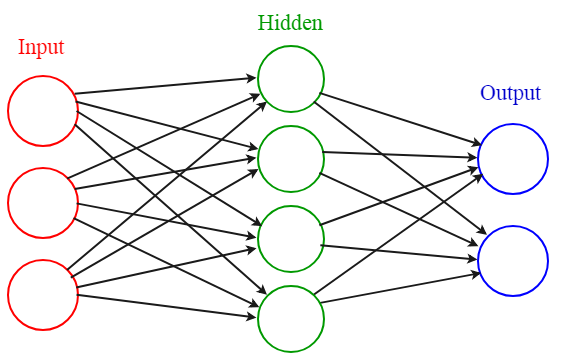
\includegraphics[height=0.35\linewidth]{./figures/feedforward}
	\caption{A neural network, where the circles represent the artificial neurons as nodes}
	\label{fig:feedforward}
\end{figure}

The artificial neural network itself is not an algorithm, but rather a framework for many different machine learning algorithms that can process complex data inputs. These learning algorithms learn from the experiences that are obtained from processing many examples. Each process yields an output, which, depending on the other outputs can determine which characteristics of the input are needed to construct the correct output. If there are a sufficient number of processed examples, the neural network can generate potential inputs and see if they produce the correct outputs. As the quantity of training data increases, so does the learning time and complexity of the neural network. However, training data also potentionally increases the estimation accuracy.



\subsection{Inversion}

There is a subfield of machine learning that is hardly researched yet, called the inversion problem \cite{KINDERMANN1990277}. \smallskip

\label{para:inversion}A properly trained neural network can model the process that is generating the training data and even the inverse process. Neural network inversion procedures seek to find one or more input values that produce a desired output response for a fixed set of synaptic weights. \medskip

There are many methods which can perform neural network inversion. These can be placed into three broad classes. Exhaustive search should be considered when the dimensionality of the input and allowable range of each input variable is low. Single-element inversion methods are used to find one inversion point per process. Multi-element inversion procedures are able to find numerous inversion points simultaneously. \medskip

Even if the inversion problem is not the most popular area in connection with neural networks, it has wide application areas. For example, a single-element inversion task is the problem of sonar performance under various environmental conditions \cite{article}. A neural network is trained to generate SIR pixel values as a function of sonar and environmental parameters. Once trained, the inverted neural network can provide input parameters to generate desired SIR performance in a specified target region. 



\section{Python}

Python is an interpreted, object-oriented, high-level programming language with dynamic semantics, used for general-purpose programming. It was created by Guido van Rossum and released in 1991. \medskip

Python has became a first-class tool over the last couple decades for scientific computing tasks, including the analysis and processing of large datasets. It is easy to learn, has efficient high-level data structures and a simple but effective approach to object-oriented programming.\medskip

In the artificial intelligence community, Python is one of the most used language. Numerous artificial intelligence fields' researchers develop in Python, with the assistance of the built-in libraries and several other sources found on the internet. The usefulness of Python for data science comes primarily from the large and active third-party packages: 
\begin{verse}
	- \textbf{Scikit-Learn} for providing a uniform toolkit for applying common machine learning algorithms to data;
	
	- \textbf{NumPy} for providing efficient storage and computating multi-dimensional data arrays;
	
	-  \textbf{Pandas} for providing a DataFrame object along with a powerful set of methods to manipulate, filter, group, and transform data; 
	
	- \textbf{Matplotlib} for providing a useful interface for creating publication-quality plots and figures;
\end{verse} 
and many more tools that aimed scientific computing and other machine learning fields. Also the vast majority of the libraries used for data science have Python interfaces.\\ 
Besides the prebuilt libraries, choosing Python for artificial intelligence programming can make the development easier and faster with the specific indenting style and the dynamic typing system, which means less coding and more developing. Python is platform independent, its interpreter and extensive standard library are available in source or binary form for free.
\chapter{Theoretical Background}

\section{Data Mining}

Data mining is a subfield of computer science and statistics that uses machine learning and statistical methods to discover patterns in large data sets. Data mining has various stages to process knowledge and all of the stages run different methods to collect the appropriate datas.\medskip

The first and most important part is to select the dataset which will be processed. This means two things. Firstly the goal needs to be drawed up. Secondly the information that seems to be useful for the goal needs to be selected. \smallskip

\noindent To decide the usefulness of a feature, it needs to pass a set of quality criteria.
\begin{verse}
	$\bullet$ Validity: the degree to which the measures conform to defined business rules or constraints\\
	$\bullet$ Accuracy: the degree of conformity of a measure to a standard or a true value\\
	$\bullet$ Completeness: the degree to which all required measures are known\\
	$\bullet$ Consistency: the degree to which a set of measures are equivalent in across systems\\
	$\bullet$ Uniformity: the degree to which a set data measures are specified using the same units of measure in all systems
\end{verse}

After the features has selected, they are just raw data and need a revision to reduce the amount of further data cleaning. There are some other criteria for the qualities of good features. \smallskip

Good feature values should appear more times in a data set. It enables a model to learn how this feature value relates to the label. This means having many examples with the same value helps the model to see the feature in different settings to determine when it is a good predictor. Also, each feature should have a clear and obvious meaning to anyone. 


\subsection{Preprocessing}

Data preprocessing is a data mining technique that involves transforming raw data into an understandable format. The selected dataset may include errors, missing values or noisy, inconsistent datas. During the preprocessing stage, these datas need to be filtered out. \smallskip

Data preparation and filtering steps can take considerable amount of processing time. Data preprocessing includes cleaning, integration and reduction. Sometimes data transformation takes place in the preprocessing too. The product of data preprocessing is the final training set.


\subsubsection{Data cleaning}

The given data in large datasets often contains information that is not clear enough. That can happen from a number of reasons. For example the data can be incomplete as lacking attribute values or certain attributes of interest. The data can be inconsistent or noisy too if it contains errors or too much outlier values that deviates from the expected. There are several techniques for repairing these useless datas.\medskip

\noindent For missing values, there are two things can be done:\\
1. Simply ignore the tuple, which is only effective if the tuple contains several missing attributes\\
2. Fill the missing values manually, that can be done with the mean value or a global constant (like $\infty$)\\
Both techniques can cause noise and inaccuracy, but the current tuple may contain important information too.\smallskip

Noise is a random error or variance in a measured variable. Noisy data needs to be smoothed to get the accurate prediction. "Binning" methods smoothes the value with its neighbour's, so it is just a local smoothing technique. Clustering can be used to detect outlier values by organizing them into similar groups. Data can be smoothed by fitting the data to a function such as regression.\smallskip

Data inconsistencies can be solved manually by external references, or with the use of knowledge engineering.


\subsubsection{Integration and Reduction}

Data integration and reduction aims on the same goal, to have a smaller dataset. During integration, an algorithm is looking through the dataset and looking for redundacies and multiple data. \medskip

Data reduction is reducing the volume or the dimension of the dataset, without compromising the integrity of the original dataset. As the analysing can be time consuming, these data reduction techniques are really helpful in large datasets:\\
1. Dimension reduction: drop the irrelevant or weakly relevant values from the dataset\\
2. Data compression: use various encoding techniques to reduce the size of the dataset


\subsubsection{Transformation and Future Scaling}

Some features of the dataset need some transformation to get an appropriate form for mining. Data transformation involves a bunch of statistical techniques, called future scaling. \smallskip

Future scaling is a method used to standardize the range of the data. The raw data have a wide range of values that can make noisy data, and in some machine learning algorithms, objective functions will not work properly without normalization. To scale the range of the datas, mathematical procedures can be used.\medskip

\textbf{Normalization} is the process of scaling individual samples to have unit norm. Min-max scaling or min-max normalization is the simplest method that rescales the range of features to $[0, 1]$ or $[-1, 1]$. Selecting the target range depends on the nature of the data. The general formula is given as:
$$ x' = \frac{x-min(x)}{max(x)-min(x)} $$
where $x$ is the original value and $x'$ is the normalized value.\\
Mean normalization is similar to min-max scaling, where $\bar x = average(x)$:
$$ x' = \frac{x-\bar x}{max(x)-min(x)} $$ \medskip

\textbf{Standardization} of datasets is a common method to transform the given data as if they comes from standard normally distributed data set. Feature standardization makes the values of each feature in the data have zero-mean and unit-variance. \smallskip
	
In practice the shape of the distribution is often ignored and just transform the data to center it by removing the mean value of each feature, then scale it by dividing non-constant features by their standard deviation.
$$ x'= \frac{x-\bar x}{\sigma} $$
where $x$ is the original feature vector, $\bar x$ is the mean of that feature vector and $\sigma$ is its standard deviation.\bigskip

\textbf{Encoding} is the process of converting data into a form that is  required for a number of information processing needs. It can be used effectively on categorical features since they have a discrete set of possible values. \smallskip

Integer encoding converts the nomimal values to numeric values, but it will impose some constraints. These numeric values are integers in increasing order, so they can be problematic during the training process. They can cause inconsistency with the given weights.\smallskip

One-hot encoding offers a solution for this problem. It creates a binary vector for each categorical feature in the model that represents values as follows:\\
$\bullet$ For values that apply to the example, set corresponding vector elements to 1.\\
$\bullet$ Set all other elements to 0.\\
The length of this vector is equal to the number of elements in that current feature set.


\subsection{Data Mining Algorithms}

After the appropriate training set is given, the following data mining techniques can be used to discover the patterns:\\
1. Classification: this method helps to classify data in different classes\\
2. Clustering: identifies data that are like each other to understand the differences and similarities between the data\\
3. Regression: this is the method of identifying and analyzing the relationship between variables\\
4. Association: it discovers a hidden pattern in the data set\\
5. Outer detection: collects the data which do not match an expected pattern or expected behavior\\
6. Sequential Patterns: this method helps to discover or identify similar patterns or trends in transaction data for certain period\\
7. Prediction: it analyzes past events or instances in a right sequence for predicting a future event \medskip

Data mining's applying techniques come from a wider field called \textbf{data analytics}. In a simple explanation data analytics is the process of examining data sets in order to draw conclusions about the information they contain. It focuses on processing and performing statistical analysis on existing data sets. A widely used data analytics technique is machine learning, because it can process data sets more quickly than it can be done via conventional analytical modeling. Machine learning automates model building, due to it relies on patterns and inferences, instead of explicit instructions.



\section{Feedforward Neural Networks}

There are many different types of neural networks, one of them is the feedforward neural network \cite{fine2006feedforward}. It aims on to create a mapping from a properly trained input dataset to an estimated output and it is able to model complex non-linear functions. \medskip

A feedforward neural networks units are the artificial neurons, that are conventionally called \textbf{nodes}. To determine the value of a node, all the inputs would be multiplied one by one with their weights, and then adding their sums. This type of neural network is called feedforward due to there are no feedback connections in which outputs of the model are fed back into itself. \medskip

A typical feedforward neural network consists of inputs, weights and an output. The \textbf{input layer} is a set of input neurons, where each neuron represents a feature in our data set. The \textbf{output} of any feedforward network is the sum of the inputs multiplied by the weights. There is an intermediate part between inputs and outputs, called hidden layers. The \textbf{hidden layer} contains those type of units which can transform the inputs into a mapping which the output layer can use. The relationship between the input and hidden layer is determined by the weights of the network. \medskip

\noindent The output of a trained feedforward neural network can be characterized by
$$ o_k = f_k(i,w) $$
where $o_k$ is the $k$th neural network output, $(i,w)$ is a vector of the weights and $f_k(\cdot)$ describes the mapping from the input to the $k$th output, where $f_k(\cdot)$ also contains the structure of the feedforward perceptron. The neural network can be trained if the input and the output are fixed and the weights are set to get the expected results. When a single scalar output can be found, $o_k$ can be replaced by $o$ and $f_k(\cdot)$ by $f(\cdot)$.



\subsection{Single-Layer Perceptron}

The perceptron is a single layer feedforward neural network \cite{tho2010perceptron}. A single-layer perceptron has only one input and output layer and no hidden layers. The input values are presented to the perceptron, and if the predicted output is the same as the desired output, then the performance is considered satisfactory and no changes to the weights are made. However, if the output does not match the desired output and then the weights need to be changed to reduce the error. \smallskip

In order to avoid unnecessary iterations, it is important to adjust the weights properly.
$$ \Delta w = \eta * d * x $$
where $\Delta w$ stands for the current weight, $\eta \leq 1$ is the learning rate which is the size of the required steps, $d$ represents the desired output and $x$ is the input data. \medskip

The sum of the inputs multiplied by the appropriate weights are led directly to the output layer. This weighted sum stands for \textbf{dot product} in this context: $ z = w_1 x_1 + w_2 x_2 + \dots + w_m x_m = \sum_{j=1}^m w_j x_j $

\begin{figure}[h]
	\centering
	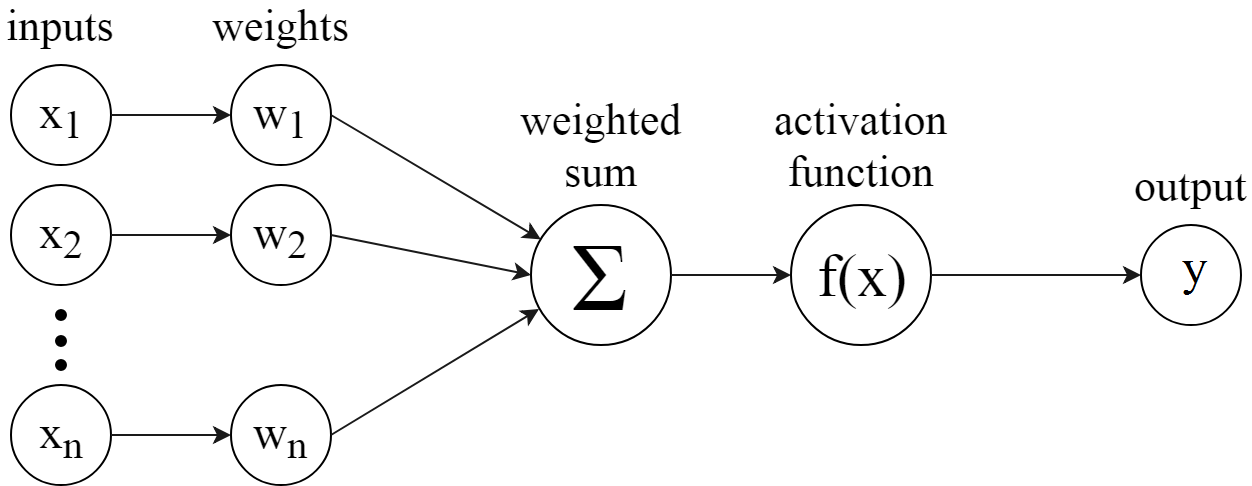
\includegraphics[height=0.28\linewidth]{./figures/perceptron}
	\caption{The appropriate weights are applied to the inputs and the resulting weighted sum passed to an activation function that produces the output.}
	\label{fig:perceptron}
\end{figure}

The output $o$ is determined by whether the weighted sum $\sum_j(w_j x_j)$ is less than or greater than some threshold value $\theta$, which is the parameter of the neuron. If that value is above a given threshold, it "fires", which means that the neuron gets an activated value. 
$$ o = \begin{cases} 0, & \hbox{for}~ \sum_j(w_j x_j) < \theta \\ 1, & \hbox{for}~ \sum_j(w_j x_j) \geq \theta \end{cases} $$



\subsection{Multi-Layer Perceptron}

The multi-layer perceptron is a supervised learning algorithm that learns a function $f(\cdot) : \mathbb{R}^m \mapsto \mathbb{R}^o$ by training on a dataset, where $m$ is the number of dimensions for input and $o$ is the number of dimensions for output. Given a set of features $X = x_1, x_2, \dots, x_m$ and a target $y$, it can learn a non-linear function approximator for either classification or regression. \medskip

The difference between single- and multi-layered neural networks that the multi-layered one has one or more hidden layers besides the input and output layer. Except for the input nodes, each node is a neuron that uses a non-linear activation function. \medskip

In a multi-layer perceptron, each neuron in one layer is connected with a weight to another neuron in the next layer. Each of these neurons stores an amount, which is in general a sum of the weighted neurons come from previous layers. There is a special unit, called \textbf{bias} units, that are not influenced by any values in the previous layer, so they do not have any incoming connections. However they have outgoing connections and they can contribute to the output of the artificial neural network. Now the definition of dot product expands like this:
$$ z = \sum_{j=1}^m w_j x_j + bias $$

A neural network was made to learn from changing the connected weights after every piece of data is processed, compared to the expected result, based on the amount of error. A multi-layer perceptron utilizes a supervised learning technique called \textbf{backpropagation} for training.


\subsubsection{Backpropagation}

The main goal of backpropagation is to update all of the weights in the neural network, so they cause the predicted output to be closer to the target output with minimizing the error of each output neuron and also the network. \medskip

The algorithm consists of two phases: the forward phase where the activations are propagated from the input to the output layer, and the backward phase, where the error between the actual and the desired nominal value in the output layer is propagated backwards in order to modify the weights values. \medskip

The function that is used to compute this error is known as \textbf{loss function}. The loss function is a function that maps values of one or more variables onto a real number intuitively representing some "cost" associated with those values. For backpropagation, the loss function calculates the difference between the network output and its expected output, after a training example has propagated through the network. \smallskip

Different loss functions will give different errors for the same prediction, and thus have a considerable effect on the performance of the model. In the training of multi-layer perceptrons, L2 loss function $L$ has been used, which is the square of the L2 norm of the difference between actual value $y$ and predicted value $\hat{y}$.
$$ L = \sum^n_{i=1}(y - \hat{y})^2 $$



\subsubsection{Gradient descent}

Backpropagation uses gradient descent in the calculation of the weights used in the neural network. It is an optimization method, which aims on to minimize a given function to its local minimum by iteratively updating the weights of the model. The input is defined with an initial value and the algorithm calculates the gradient i.e. the partial derivative of the loss curve at this starting point. \smallskip

\noindent The components of gradient descent are the following:
\begin{verse}
	$\bullet$ Learning rate: size of steps took in any direction\\
	$\bullet$ Gradients: the direction of the steps, i.e. the slope\\
	$\bullet$ Cost function: tells the current height, which is the sum of squared errors
\end{verse}

\begin{figure}[h]
	\centering
	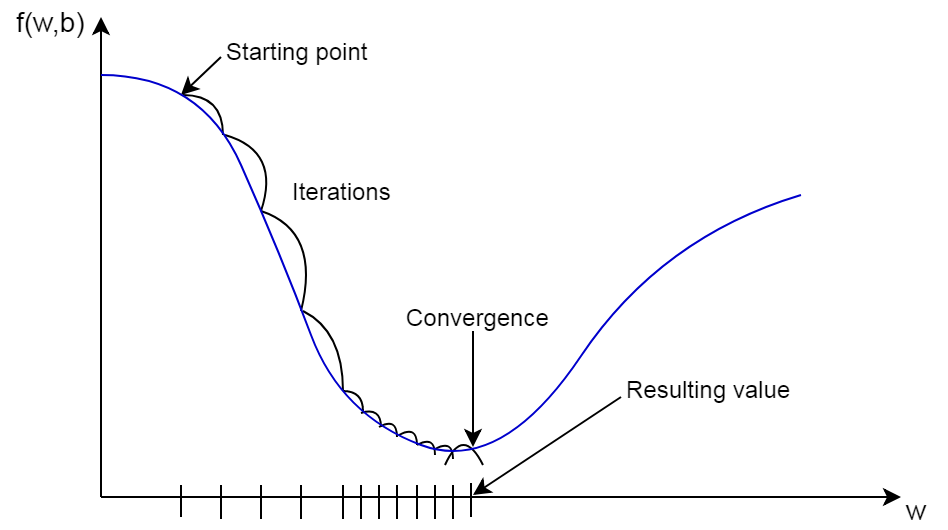
\includegraphics[height=0.35\linewidth]{./figures/gradient}
	\caption{The gradient descent is an optimization method used by backpropagation}
	\label{fig:gradient}
\end{figure}

In backpropagation, the calculation of the gradient proceeds backwards through the network, so the partial computations of the gradient from one layer are reused in the computation of the gradient for the previous layer. This backward phase is a more efficient way of computing the gradient at each layer, instead of calculating the gradient of each layer separately.



\section{Training a MLP Model}

The task that is being tackled in this paper is to make the inversion of a single-element feedforward neural network. To result this successfully, the appropriate dataset is given and already preprocessed. Hence the main task is now to train a neural network to predict new outputs for the testing set and minimize the loss between the given and the desired outputs from the training set. \medskip

The components of a neural network model i.e the activation function, optimization algorithm and the size of the layers play a very important role in effectively training a model and produce accurate results. Different tasks require a different set of functions to give the most optimum results. The used methods and functions are described in the following.


\subsection{Regression}

Regression is a supervised learning task of machine learning that is used to predict values of a desired target variable. It is a statistical technique which requires a data set with the desired output that is consists of one or more continuous variables and real numbers.\smallskip

Using regression the input vector is mapped onto a given set of values by the network. The network regresses the independent variables, provided by the inputs, onto the dependent variable. The multi-layer perceptron uses non-linear regression.  \medskip

In a linear regression task there is one independent variable $x$, to explain or predict the outcome of the dependent variable $y$.
$$ y = \beta_0 + \beta_1x + \epsilon $$
where $\beta_0$ stands for the intercept, $\beta_1$ is the steep of the independent variable and $\epsilon$ represents the error value that is the residual of the regression. \medskip

In non-linear regression, a statistical model of the form is
$$ y \approx f(X,\beta) $$
that relates a vector of independent variables $X$, and its associated observed dependent variables $y$. The function $f$ is non-linear in the components of the vector of parameters $\beta$, but otherwise arbitrary. 



\subsection{Activation Functions}

In artificial neural networks, the activation function is a transitional state of the neurons between other layers. It is a mapping of the previous layers and it maps the resulting value into the desired range, which is usually between -1 and 1. The output of the activation function is then used as input for the next layer, until a desired solution is found. There are several activation functions, and each of them utilizes different algorithms for mapping. \smallskip

As the multi-layer perceptron applies non-linear approximator functions, it will be the most accurate by using non-linear activation functions as well. They are known about having more than one degrees and they have a curve in their graph. Due to non-linear functions can generate non-linear mappings from inputs to outputs, they can be applied in complex data sets. 

\begin{figure}[h]
	\centering
	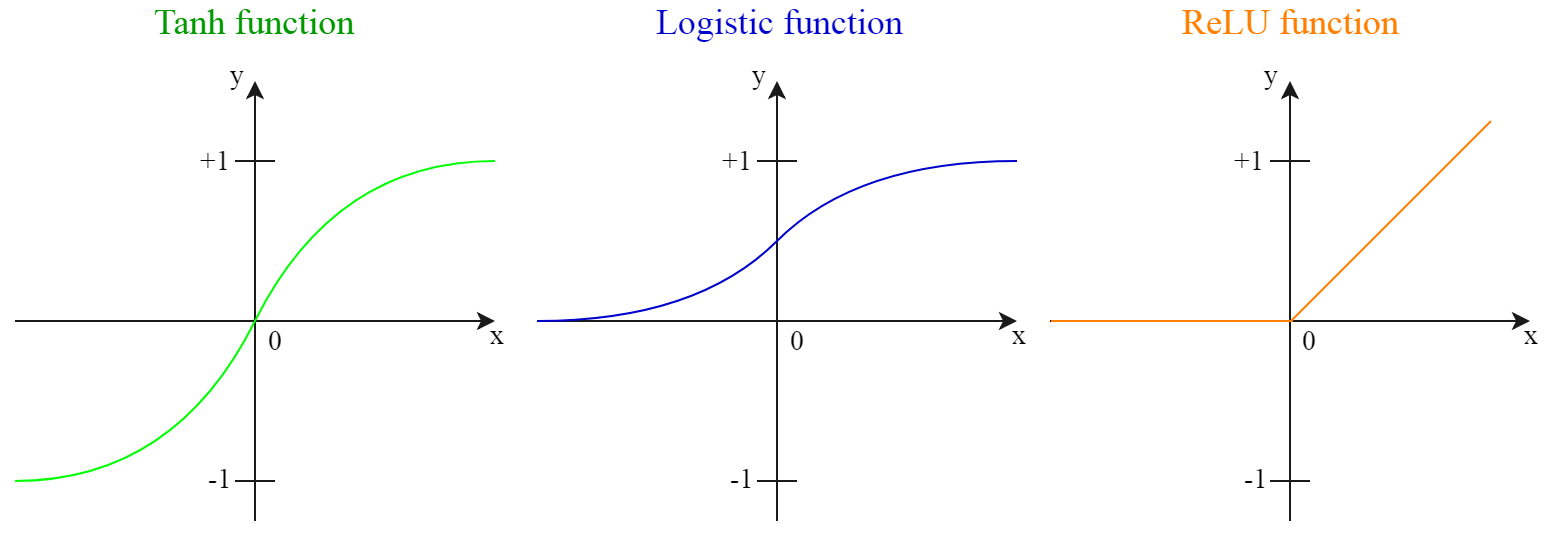
\includegraphics[height=0.35\linewidth]{./figures/functions}
	\caption{The graphs of the most popular non-linear activation functions}
	\label{fig:functions}
\end{figure}

The two common activation functions are both sigmoids, and are described by
$$ f(x)=tanh(x) ~~~ \hbox{and} ~~~ f(x)=\sigma (x)=\frac{1}{1+e^{-x}} $$
The first is a \textbf{hyperbolic tangent} that ranges from -1 to 1, while the other is the \textbf{logistic} function, which is similar in shape but ranges from 0 to 1. \smallskip

The \textbf{ReLU} function is another type of non-linear functions, which stands for rectified linear unit. Its is called half-rectified, due to if the data set consists any negative values, that will turn into 0 immediately. This operation affects the resulting graph (\autoref{fig:functions}), due to the appropriate values will not be mapped.
$$ f(x) = \begin{cases} 0, & \hbox{for}~ x < 0 \\ x, & \hbox{for}~ x \geq 0 \end{cases} $$



\subsection{Optimization Methods}

Artificial neural networks have different phases in the process of their operation. The procedure of the learning process in a neural network can apply different training methods with different characteristics and performance. These training methods use optimization algorithms to update weights and biases i.e. the internal parameters of a model to reduce the error. \cite{veerarajan2007numerical}\cite{pillo2013nonlinear}



\subsubsection{Stochastic Gradient Descent}

\begin{figure}[h]
	\centering
	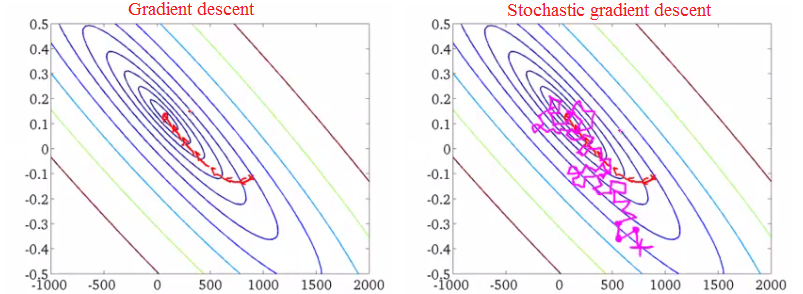
\includegraphics[height=0.28\linewidth]{./figures/stochastic}
	\caption{The difference between the process of GD and SGD methods}
	\label{fig:stochastic}
\end{figure}
Stochastic gradient descent \cite{Bottou2012} is a stochastic approximation of gradient descent optimization, used effectively in large-scaled data sets. It can also work in a system of linear and non-linear equations and can effectively solve unconstrained optimization problems. In constrant to gradient descent, the stochastic method can approximate the true gradient of the cost function because it updates the parameters for each training example, one by one. To demonstrate assume that $\eta$ is the learning rate, $L$ stands for the loss function and $\nabla_w L = \frac{\partial L}{\partial w}$ is the gradient. Now the update equation of the weights $w$ in each iteration is:
\begin{equation} w_{t+1} = w_t - \eta \nabla_w L \label{eq:sgd} \end{equation} 

\noindent The process of the stochastic gradient descent algorithm is the following:\\
1. Choose one sample from the dataset (this is what makes it stochastic gradient descent).\\
2. Calculate all the partial derivatives of loss with respect to weights or biases. \\
3. Use the update equation \eqref{eq:sgd} to update each weight and bias.\\
4. Go back to step 1.


\subsubsection{Adam}

Another method is Adam, whose name is derived from adaptive moment estimation. It is a transition between adaptive methods and momentum-based methods. In the algorithm, running averages of both the gradients and the second moments of the gradients are used, which means Adam not just stores the exponentially decaying average of past squared gradients $v_t$, it also keeps the decaying average of past gradients $m_t$, similarly to momentum-based methods. The algorithm computes the decaying averages of past $m_t$ and past squared $v_t$ gradients respectively as follows:
$$ m_t = \beta_1 m_{t-1} + (1-\beta_1)L_t ~~~~\hbox{and}~~~\ v_t = \beta_2 v_{t-1} + (1-\beta_2)L^2_t $$
where $m_t$ and $v_t$ are the estimates of the first and second moments, $\beta_1$ and $\beta_2$ are the decay for gradients and second moments of gradients, and $L_t$ is the loss function.\\
The first and second moment estimates are:
$$ \hat{m_t} = \frac{m_t}{a-\beta^t_1} ~~~~\hbox{and}~~~ \hat{v_t} = \frac{v_t}{a-\beta^t_2} $$
Then these estimates are used to update the parameters $w$ with a simple scalar $\epsilon$ to prevent division by 0
$$ w_{t+1} = w_t - \frac{\mu}{\sqrt{\hat{v_t}}+\epsilon}\hat{m_t} $$


\subsubsection{Limited-memory BFGS}

Limited-memory BFGS is an approximation of Broyden–Fletcher–Goldfarb–Shanno (BFGS) algorithm, which is an iterative method for solving unconstrained non-linear optimization problems. The difference between them, that L-BFGS uses a limited amount of computer memory. It aims on parameter estimation, and the target problem is to minimize $f(x)$ over unconstrained values of the real-vector $x$ where $f$ is a differentiable scalar function. In this method, the Hessian matrix of second derivatives is not computed, but it is approximated by using gradient evaluation updates. \medskip

\noindent From an initial guess $x_0$ and an approximate Hessian matrix $B_0$, the following steps are repeated as $x_k$ converges to the solution:\\
1. Obtain a direction $p_k$ by solving $B_k p_k = - \nabla f(x_k). $ \\
2. Perform a one-dimensional optimization to find an acceptable stepsize $\alpha_k$ in $p_k$. \\
3. Set $s_k = \alpha_k p_k$ and update $x_{k+1} = x_k + s_k.$ \\
4. Set $y_k = \nabla f(x_{k+1}) - \nabla f(x_k).$ \\ 
5. The solution is $B_{k+1} = B_k + \frac{y_k y^T_k}{y^T_k s_k} - \frac{B_k s_k s^T_k B_k}{s^T_k B_k s_k}.$

\begin{figure}[h]
	\centering
	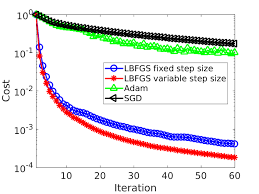
\includegraphics[height=0.34\linewidth]{./figures/optimization}
	\caption{The optimization of SGD, Adam and L-BFGS with respect of cost and iteration}
	\label{fig:optimization}
\end{figure}





\section{Inversion}

As mentioned in \autoref{para:inversion}, a properly trained neural network can model the process that is generating the training data and the inverse process too. Inversion of a neural network consists of clamping the weights and the neural network output while adjusting the input in the neural network until an equality or a best possible fit occurs for one or more values of the input. \medskip

Feedforward neural networks aim on to capture system mapping from training data. The goal is to find the input values that will result the desired output for the given synaptic weights. Generally it can be determined that a single input can generate numerous outputs. \smallskip

\noindent The process is the following:\\
1. Fix the weights and the outputs.\\
2. Find such an input that concurs or mostly fits the supposed input. \medskip

\noindent To achieve the goal, it is necessary to:\\
1. find every point that can fit the input\\
2. define the external points as thresholds\\
3. the evenly distributed points can be located in the solution set.



\subsection{Single-Element Inversion}

In the task of single-element inversion only one point is found by the algorithm depending on the initialization. This means it will result a nearer outcome in further processes. Hence it is very important to find a properly training algorithm, because it notes the previously founded points and reuse them. This process is very time consuming. As the quantity of parameter combinations increases during the training phase, so does the time that the training takes. However, the number of parameter combinations also potenionally increases the inversion accuracy.



\subsection{Inversion Methods}

To solve the inversion of an unconstrained optimization problem, the inversion method needs to solve the optimization itself in its training phase. After the dataset is properly trained, the inversion problem is the following:

Given some network function $f : X \mapsto Y$, for some $y \in Y$, the appropriate $x \in X$ needs to be found, such that $f(x) = y$. Or more generally, if $L : Y \mapsto \mathbb{R}$ is the loss function defined over the network output, an input $x$ have to be found that minimizes $L(f(x))$. \smallskip

Some applications have been proposed that rely on single-element inversion methods.


\subsubsection{WLK Inversion}

The WLK inversion was named after R. L. Williams, A. Linder and J.
Kindermann, who firstly introduced the single-element search method for inversion of real valued neural network. In this algorithm, the inversion problem is set up as an unconstrained optimization problem and solved by gradient descent, similarly to backpropagation. \medskip

\noindent The method of WLK inversion involves two main steps: \\
1. \textbf{training} the network \\
2. \textbf{inversion}\medskip

During the training, the neural network is trained to learn a mapping from input to output. The proper set can be find by minimizing the loss. Thus the neural network learns a functional relationship between the inputs and the outputs. Now all the weights are fixed. After the training, the network is initialized with a random input vector. Output is calculated and compared with the given output. Now the error can be calculated and backpropagated to minimize the loss function and the input vector is updated. This iterative process continues until the error is less than the minimum set value.\medskip

Assume that the initial input vector $i_0$ is given. Now the recursive equation of the training phase is the following: 
\begin{equation} i_k^{t+1} = i_k+t - \eta \frac{\partial E}{\partial i_k^t} \label{eq:wlk} \end{equation} 
$t$ - the index of the iteration, \\
$i_k^t$ - the $k$th component of the $i^t$ vector, \\
$\eta$ - the learning rate \medskip

Due to the general feedforward topology, the iteration for inversion in \eqref{eq:wlk} can be solved by the dervative of 
$$ \frac{\partial E}{\partial i_k} = \delta k ~~~~ k \in I$$
for every $\delta k$:
$$ \delta j = \begin{cases} \varphi'_j(o_j)(o_j-t_j):, & ~ j \in O \\ 
\varphi'_j(o_j)\sum_{m\in H,O}\delta_j w_{jm}:, & j \in I, H \end{cases} $$

\noindent $I, O, H$ - the set of input, output and hidden neurons,\\
$w_{jm}$ - the weight value from neuron $j$ to neuron $m$,\\
$\varphi'_j$ - the derivative of the $j$th neuron squashing function,\\
$o_j$ - the activation of the $j$th neuron,\\
$t_j$ - the desired output of the $j$th neuron \medskip

The derivatives of the neurons need to be solved by backward order from the output to the input. Thus everything is given in the equation, but the absence of feedback, so the relationship of the neurons is only an assumption.


\chapter{Implementation}

This work belongs in the realm of machine learning application research. There are three main tasks examinated in this paper: data mining for extracting information from a data set, building and testing multilayer perceptron models for, and inverting these feedforward neural network models. \medskip

The first task is to choose a dataset which contains usable data. The selected one is called the Online News Popularity Dataset by Mashable news, that was served by the  \href{http://archive.ics.uci.edu/ml/datasets/Online+News+Popularity}{UCI's Machine Learning Repository}. \smallskip

The dataset is preprocessed by Pandas to get is ready for data mining. Since being a publicly available dataset, its preprocessing and transformation has already made, but the dataset even needs some cleaning, like scaling, with the assistance of Scikit-Learn. Then the training set is made for the training.\smallskip

The training phase consists of the application of machine learning techniques. With the utilization of the inputs, Scikit-Learn trains the training dataset and make predictions to the testing set. The training is very time consuming, since the used dataset is very large, and also the length is depending on the amount of attributes of multi-layer perceptron models. In the end of each process, the testing set's output and the predicted output are compared and the difference between them is calculated. If all of the iterations are ended, the best estimator's parameters are shown with its score, and the tested target values and the predicted ones are plotted by Matplotlib.\smallskip

From the results of the training, the single-element inversion can be performed by Scikit-Learn. It is an iterative process, where the target values are the new predictors with the knowledge comes from the other features. Every iteration calculates one single feature's values and also its accuracy between the feature's original and the calculated values. The results are also plotted by Matplotlib. \smallskip

These results show the influence of the features to the target. The larger the score, the more important the feature is.



\section{Python}

Python can be used effectively with the assistance of some of its third-party libraries \cite{g2015learning} \cite{bressert2012scipy}, which provide numerous effective and easy-to-use models in scientific research. 


\subsection{Training Libraries}

Scikit-Learn is a free Python package, that is a separately-developed and distributed third-party extension to SciPy. It integrates classic machine learning algorithms into the scientific Python packages. Scikit-Learn can be used to solve multi-layer neural network learning problems. Among many others, it features various classification, regression and clustering algorithms.

\todo{more libraries, descriptions}


\subsection{Inversion Libraries}

asd




\section{The Implementation (?)}

\todo{new section name (?)}


\subsection{Optimising/Analysing the Dataset (?)}

asd


\subsection{Training the Neural Network}

asd


\subsection{Inverting the MLP}

asd




\section{Results}

asd
\chapter{Summary}

\todo{megirni}

\bibliographystyle{plain}
\bibliography{references}

\appendix

\chapter*{Media Instruction Manual}



\end{document}